\documentclass{article}
\usepackage{mystyle}

\title{Notes on HARDI data preprocessing}
\author{Scott Trinkle}
\date{Last edited: \today}

\begin{document}
\maketitle

\section{Introduction}
This report describes the steps in preprocessing the HARDI mouse data. Namely,
it details the application of a denoising algorithm and the spatial registration
of the data acquired with different diffusion weightings.

\section{Denoising}
The denoising algorithm comes from a paper by Veraart \textit{et al}
\cite{Veraart2016b}, and is implemented in the
\href{https://mrtrix.readthedocs.io/en/latest/reference/commands/dwidenoise.html#dwidenoise}{MRtrix3
  software package}, written by the Tournier group.

\subsection{Denoising method summary}
Consider a real-valued, redundant dMRI data matrix $\bm{X}$, with $M$ rows
representing different diffusion-weighted measurements and $N$ columns
representing voxels within a local neighborhood. The assumption of data
``redundancy'' amounts to the assumption that the data can be synthesized by a
small number, $P \ll \text{min}(M, N)$ of principal components. Veraart shows in
another paper \cite{Veraart2016a} that the oversampling of $q$-space in dMRI
leads to sufficient redundancy.

Principal components of $\bm{X}$ can be derived via singular value
decomposition of $\bm{X}$:
\begin{align}
  \bm{X} = \sqrt{N}\bm{U}\bm{\Lambda}\bm{V}^T,
\end{align}
where the singular value, $\Lambda_{ii}^2 = \lambda_i$ is the $i$th
eigenvalue of the $M\times M$ matrix:
\begin{align}
  \bm{\Sigma} = \frac{1}{N}\bm{X}\bm{X}^T.
\end{align}

A note on notation: the paper assumes $M < N$ for the purposes of the
derivation, though that choice is arbitrary, and is obviously not the case for
our data.

Noise will generally make all $M$ eigenvalues of $\bm{\Sigma}$ nonzero. In
agreement with an asymptotic universal law resulting from random matrix theory
for noisy covariance matrices, the $\tilde{M} = M - P$ smallest nonzero
eigenvalues are described by the Marchenko-Pastur (MP) distribution if the noise
level is constant among all elements of $\bm{X}$ \cite{Marchenko1967}:
\begin{align}
  p(\lambda, \sigma, \gamma) =
  \begin{cases}
    \frac{\sqrt{(\lambda_+ - \lambda)(\lambda - \lambda_-)}}{2\pi\gamma\lambda\sigma^2} & \text{if } \lambda_- \le \lambda \le \lambda_+\\
    0 & \text{otherwise,}
  \end{cases}
\end{align}
where
\begin{align}
  \lambda_{\pm} &= \sigma^2(1 \pm \sqrt{\gamma})^2,\\
  \gamma &= \tilde{M} / N,
\end{align}
and $\sigma^2$ is the noise variance.

The distribution edge $\lambda_+$ distinguishes between noise- and
signal-carrying principal components. The matrix can thus be denoised by
nullifying all $\lambda \le \lambda_+$, setting
$\bm{\Lambda}\rightarrow\tilde{\bm{\Lambda}}$ accordingly, and reconstructing
the matrix from the SVD:
\begin{align}
  \hat{\bm{X}} = \sqrt{N}\bm{U}\tilde{\bm{\Lambda}}\bm{V}^T.
\end{align}
This method \textbf{assumes the noise level to be constant and uncorrelated within
  the local neighborhood and across the dMRI measurements.} We need to think
about whether these assumptions hold given the time duration of our scan. 

The rest of the paper is spent deriving and testing an algorithm for
simultaneously estimating the noise level $\sigma$ and the number of significant
signal components $P$. This algorithm is implemented in MRtrix3. 

\subsection{Implementation}
The only tunable parameter available from the MRtrix3 implementation is $N$: the
size of the local sliding window used to define each $\bm{X}$. Veraart
\textit{et al} suggest choosing $N > M$, but note: ``in case of spatially
varying noise, it might be beneficial to select a sliding window with
$N \gtrsim M$.'' To test, I denoised the data with windows of size
$5 \times 5 \times 5$ ($N = 125$), $7 \times 7 \times 7$ ($N = 343$) and
$9 \times 9 \times 9$ ($N = 729$). Note that $M=160$ for our data (16 $b_0$
volumes and 144 diffusion-weighted volumes). Sample denoised slices from a $b_0$
and a diffusion-weighted image (DWI) are shown in Figure~\ref{fig:denoise_demo}
below.

\begin{figure}[h]
  \centering
  \begin{tabular}{l c c c}
     & Raw & Denoised & Raw - Denoised\\
    $b_0$ & \raisebox{-0.5\height}{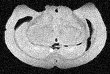
\includegraphics[width=0.3\linewidth]{figs/raw_k7_n8_sl65}} & \raisebox{-0.5\height}{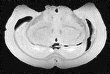
\includegraphics[width=0.3\linewidth]{figs/denoised_k7_n8_sl65}} & \raisebox{-0.5\height}{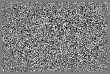
\includegraphics[width=0.3\linewidth]{figs/noise_k7_n8_sl65}}\\
      &   &   &  \\
    DWI & \raisebox{-0.5\height}{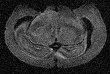
\includegraphics[width=0.3\linewidth]{figs/raw_k7_n50_sl65}} & \raisebox{-0.5\height}{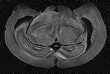
\includegraphics[width=0.3\linewidth]{figs/denoised_k7_n50_sl65}} & \raisebox{-0.5\height}{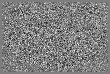
\includegraphics[width=0.3\linewidth]{figs/noise_k7_n50_sl65}}\\
  \end{tabular}
  \captionsetup{width=0.9\linewidth}
  \caption{Top and bottom demonstrate denoising of a $b_0$ and diffusion
    weighted volume, respectively. Left, center and right are the raw,
    denoised, and subtracted images, respectively. Note the lack of identifiable
    anatomical structure in the subtracted images. These images were processed
    using a $7 \times 7 \times 7$ sliding window.}
  \label{fig:denoise_demo}
\end{figure}

As a first-pass check, it is promising that no anatomical structure is visible
in the subtracted images for either the $b_0$ or diffusion-weighted
images. These sample images were calculated using a $7\times 7 \times 7$ sliding
window; there was also no structure visible for the other widths.

\section{Registration}
Minor drifts in the $B_0$ field across the 16-day scan cause slight, linear
position shifts across the different DWI. The data were acquired with 1
$b_0$ image after every 9 DWI, for a total of 16 $b_0$'s and 144 DWIs. The
registration strategy was to first register the 16 $b_0$'s, average them to
generate a mean $\bar{b}_0$, then register the 144 DWIs to $\bar{b}_0$. All
registrations were affine, calculated with the
\href{https://fsl.fmrib.ox.ac.uk/fsl/fslwiki/FLIRT}{FLIRT} \cite{Jenkinson2001,
  Jenkinson2002} tool in FSL (this was based on Sean's recommendation).


\subsection{$b_0$ registration}
The $b_0$'s were registered using a correlation-based cost function (appropriate
since we expect the same contrast for each $b_0$). I investigated two FLIRT
parameters to modify to tune the registration: affine degrees of freedom, and
voxel-weighting. The data denoised with a $7\times 7 \times 7$ window width
were used to determine optimal parameters. 

All $b_0$'s were registered to the 8th volume. Of note: there are certain
structures that appear in the first 4 $b_0$ volumes that do not appear
in the later ones. This is demonstrated in Figure~\ref{fig:b0problem}. It
is unclear to me why this happened, I need to discuss it further with Sean. 

\begin{figure}[h]
  \centering
  \begin{tabular}{c c}
    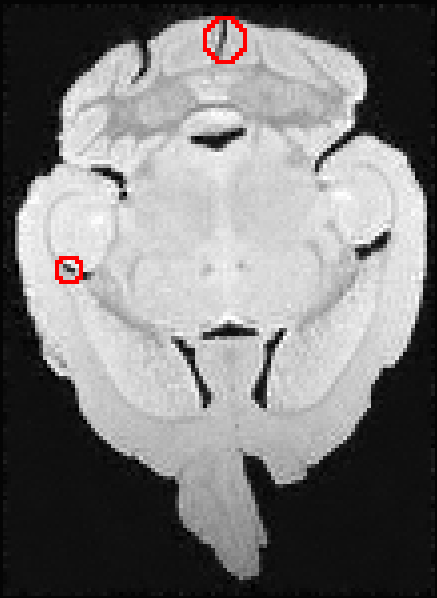
\includegraphics[width=0.3\linewidth]{figs/n0_sl36.png} & 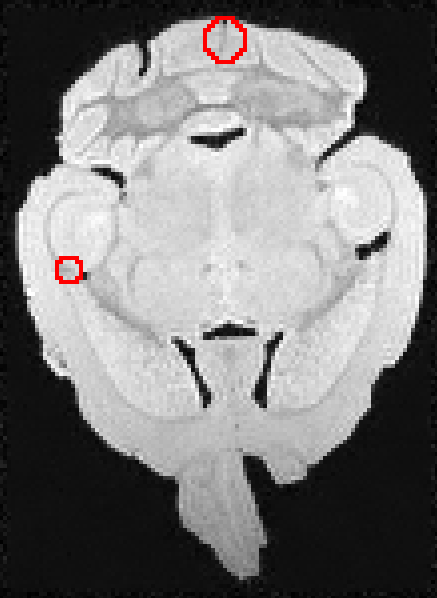
\includegraphics[width=0.3\linewidth]{figs/n8_sl36}\\
    $b_0$ \#0 & $b_0$ \#8
  \end{tabular}
  \caption{Evidence of structures in earlier $b_0$ volumes that does not appear in later volumes.}
  \label{fig:b0problem}
\end{figure}

Figure~\ref{fig:b0_dof_results} shows the performance of the registrations as a
function of affine degrees of freedom. The x-axis shows the $b_0$ volume number,
and the y-axis shows the pearson correlation coefficient between the voxels of
the registered volume and the reference volume (\#8). The dotted lines indicate
the average correlation coefficient for each curve. We see that the additional
structures in the earlier volumes negatively impact the relative registration
accuracy. Overall, using all 12 degrees of freedom had the best performance.

\begin{figure}[h]
  \centering
  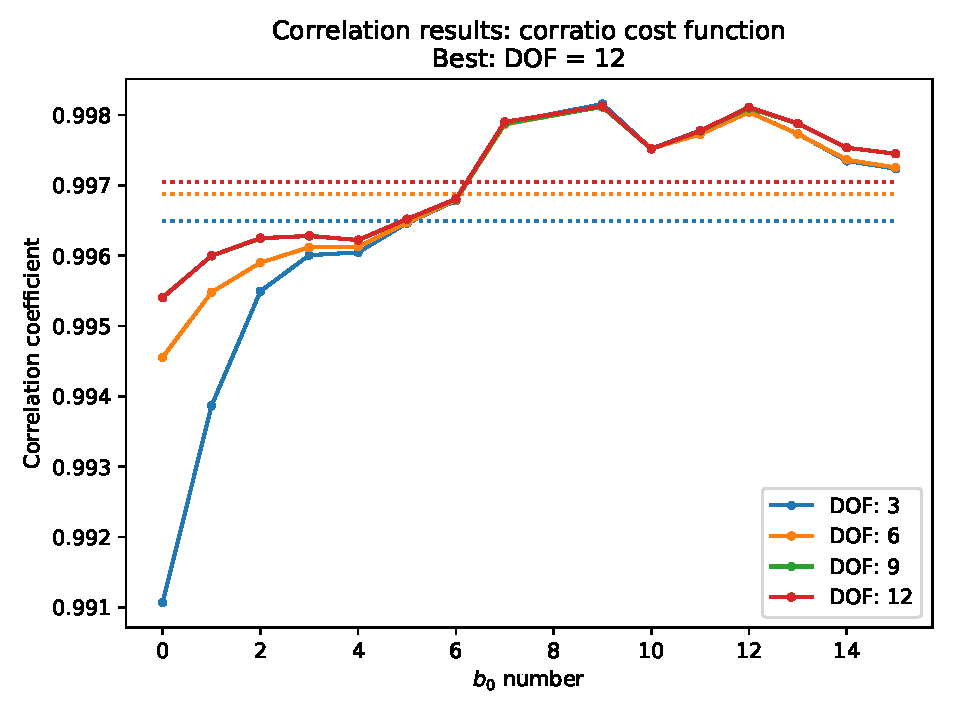
\includegraphics[width=0.5\linewidth]{figs/b0_corr_results}
  \captionsetup{width=0.7\linewidth}
  \caption{Selection of optimal $b_0$ DOF. Note the worse performance
    in the earlier volumes with the additional structures}
  \label{fig:b0_dof_results}
\end{figure}

FLIRT also allows you to input an image to use as weights for each voxel in the
optimization. Using 12 degrees of freedom, I experimented with using the reference
image (\#8) and the first image (\#0) as voxel weights. The reasoning was that
both images would weight object voxels higher than background, while the
\#0 image would place a lower weight on the additional structures, since they have
lower intensity. Figure~\ref{fig:b0_weight_results} shows the results of these
two weighting schemes compared to an non-weighted registration. 

\begin{figure}[h]
  \centering
  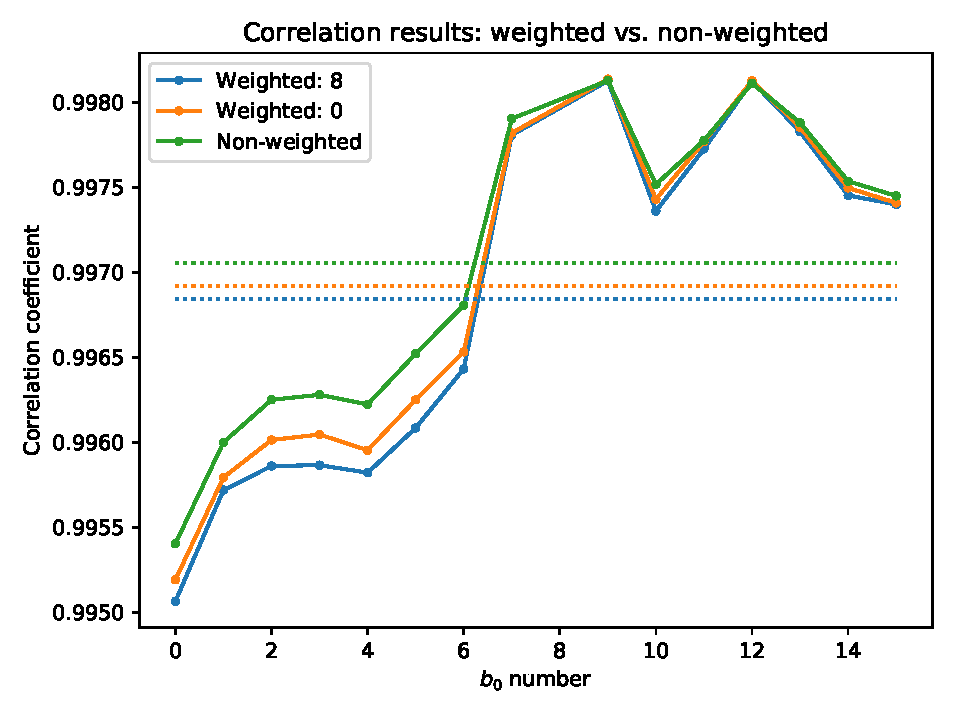
\includegraphics[width=0.5\linewidth]{figs/b0_weighted_vs_nw_results}
  \caption{Selection of $b_0$ weighting parameters.}
  \label{fig:b0_weight_results}
\end{figure}

The unweighted registration performed better for all individual volumes. Accordingly,
I decided to use an unweighted, 12-DOF affine registration for all $b_0$ volumes.

\subsection{DWI Registration}
Since the DWIs necessarily have different contrast for the same structures, they
were registered using a mutual information cost function. The strategy was to
average the registered $b_0$ volumes into a single $\bar{b}_0$, then use that as
a reference for the DW volumes. Again, I investigated affine degrees of freedom
and voxel weighting to tune the registration. Figure~\ref{fig:dwiresults} shows
the mutual information results for varying degrees of freedom and voxel
weightings. For this study, voxel weighting was done with $\bar{b}_0$. 

\begin{figure}[H]
  \centering
  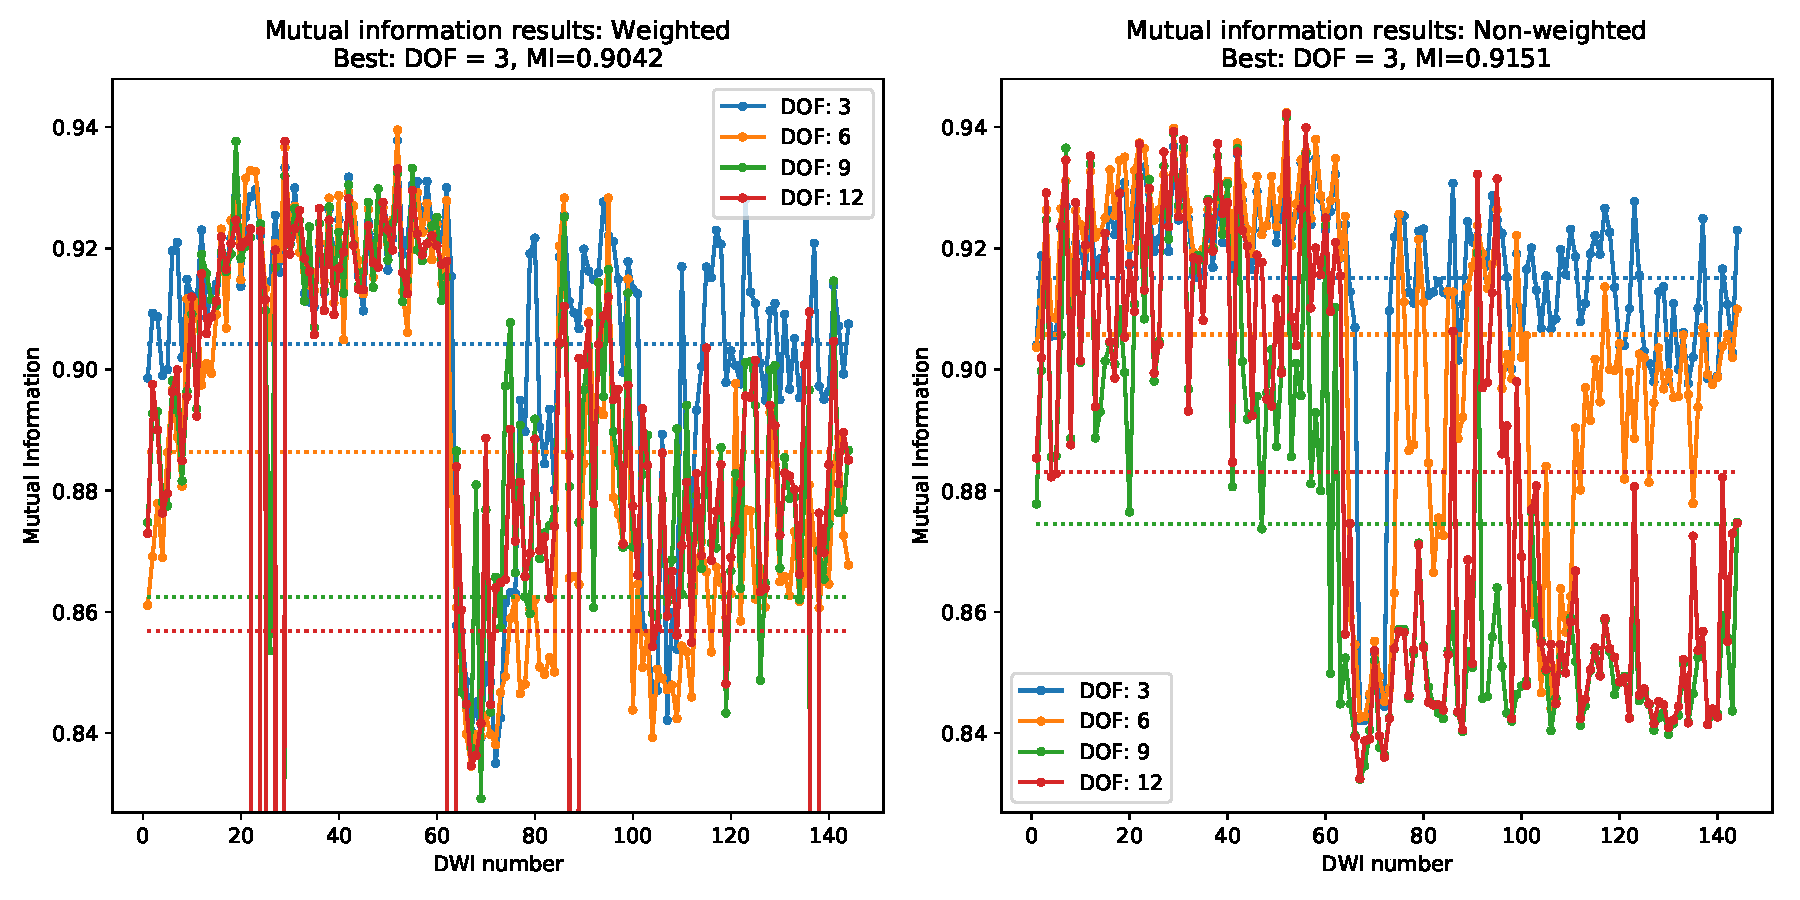
\includegraphics[width=0.9\linewidth]{figs/dwi_MI_results}
  \caption{Diffusion-weighted image registration results.}
  \label{fig:dwiresults}
\end{figure}

In general, using 3 degrees of freedom (equivalent to a rigid translation)
performed the best. Voxel weighting generally degraded performance;
using 3 degrees of freedom with no voxel weighting resulted in the best
registration overall.

\section{Conclusion}
The raw data, as well as the data denoised with the three different sliding
window widths were registered using the strategy and optimal parameters
described above. The next report will detail the effect of denoising on ODF
reconstruction, as well as exploring ODF sensitivity to sliding window width.

\bibliographystyle{ieeetr}
\bibliography{refs}
\end{document}